%!TEX root = /Users/Nikolaj/Developer/GPU-Project/Report/Report.tex

Now that it has been established that the solution produces satisfactory results it is time to examine the increase in speed the solution provides. Four different performance test was performed each one providing a different insight into how this solution was improved compared to original C\#. The graphs depicted in this section are all from the Gpulab06 machine but full performance tests for all machines can be found in (INDSÆT APPENDIX). \\

TODO: Husk at nævne at middle stepsize er altid 2 i alle test

\subsection{Variable $x$}
While changing the $x$ values should only change the runtime with a factor, it is important to show that our solution is fast no matter what values are chosen. Changing $g$ and $r$ will have no performance effect and is therefore not included in the tests.

\begin{figure}
\begin{center}
	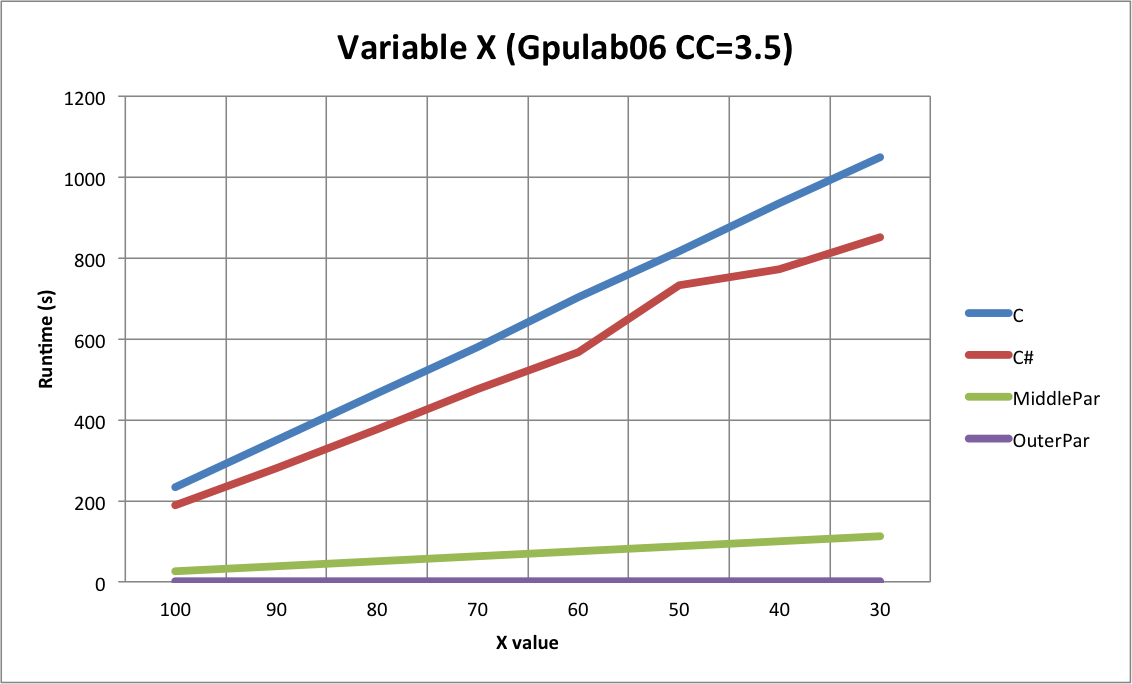
\includegraphics[width=\textwidth]{img/Gpulab-varx35.png}
\end{center}
\caption{The impact of changing the $x$ value on the Gpulab06 machine}
\end{figure}

When the $x$ value rises the runtime naturally increases because the outer model is solved from $120-x$ to 0. The lower the $x$ value the more steps needed. Our OuterPar solution is superior to all the other solution when comparing runtime, and even though the runtime also increases for this solution it is still a favorable runtime. The results showed up to 665 times faster runtime compared to the original C\# solution.

\subsection{Variable Stepsize}
One of the advantages of using a Runge Kutta 4th order solver is that an appropiate stepsize can be chosen beforehand, enabling users to get the precision they desire at the cost of runtime. While increasing the stepsize will increase the runtime in our solution the increase is quite small compared to the increase found in both the C and C\# solutions.

\begin{figure}
\begin{center}
	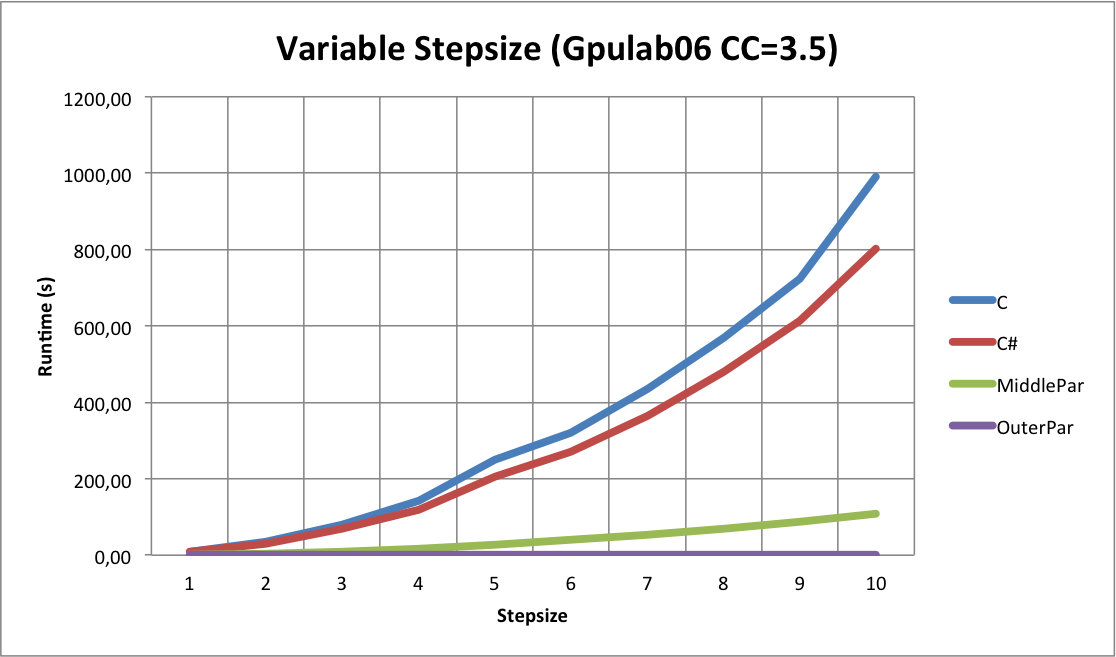
\includegraphics[width=\textwidth]{img/Gpulab-stepsize35.png}
\end{center}
\caption{The impact of changing the stepsize on the Gpulab06 machine}
\end{figure}

Increasing the stepsize does increase the runtime as expected but our OuterPar solution is superior in every test we performed on all the machines. The results showed up to 680 times faster runtimes compared to the original C\# implementation.

\subsection{Variable Threads per Block}
Since the number of threads per block is set at compile time in the CUDA solution it is interesting to test what impact different amounts have on the performance.

\begin{figure}
\begin{center}
	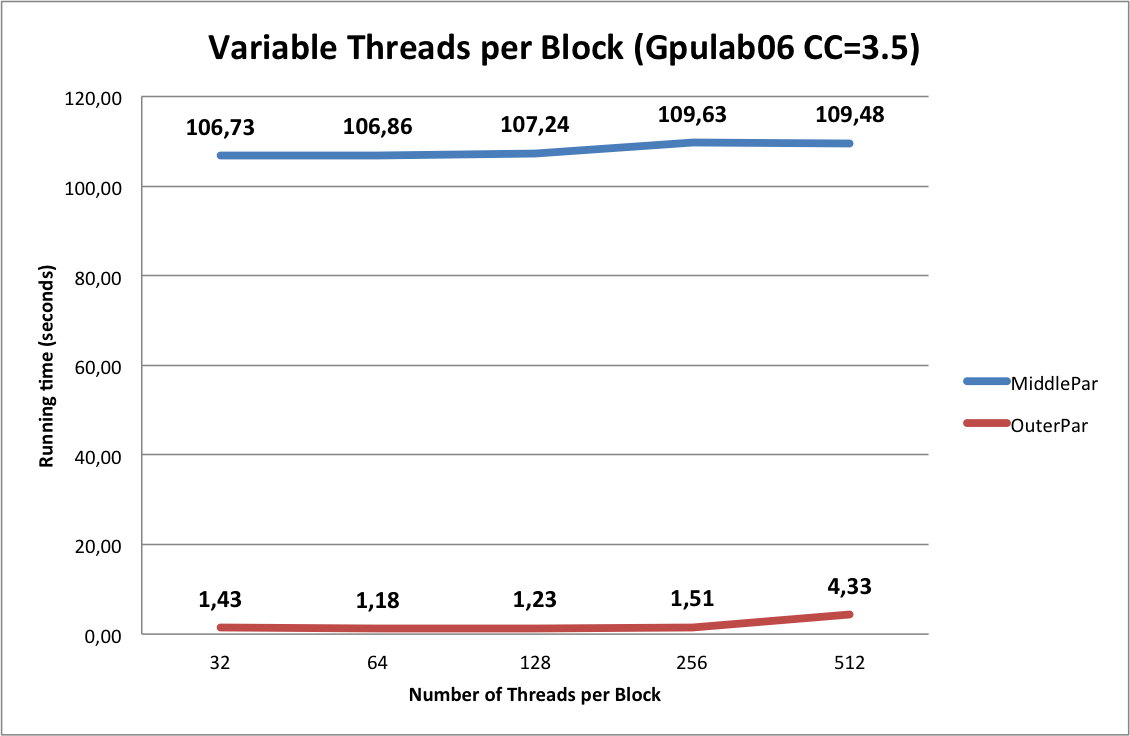
\includegraphics[width=\textwidth]{img/Gpulab-tpb35.png}
\end{center}
\caption{The impact of changing the threads per block on the Gpulab06 machine}
\label{ThreadsPerBlockGraph}
\end{figure}

\noindent As seen in Fig. \ref{ThreadsPerBlockGraph}, the slowest configuration is 512 threads per block. This is expected since the Gpulab06 GPU has a hardware limit of 2048 threads per SMP meaning that it schedules (2048 / 512) = 4 blocks at a time even though the hardware can schedule as many as 16. To increase performance, the amount threads per block has to be lowered to yield more blocks and thus a better utilisation of the SMPs. This fact explains the drastic improvement from 512 to 256 and from 256 til 128, at which the number of blocks reaches the exact hardware limit. Lowering the count further to 64 threads per block, however, seems to keep improving performance even though we already reached 16 blocks. 

In this case, the explanation should be sought in the way SMPs divide threads of the executing blocks into warps. With a configuration of 64 threads per block, the SMP splits each block into 2 warps of 32 threads each instead of 4, 8 or 16 warps with 128, 256 and 512 threads per block respectively. The lower amount of warps that each block is split into, the fewer warps will have to leave the SMP when a single thread from some block is taking long time to execute and cause the entire block to leave the SMP. This results in a faster exchange of blocks which means that the amount of threads in an SMP that is actually doing some work increases.\\

TODO:
Afrunding på hele B\&C (også afvigelser i middlepar på NSJ)

\subsection{Register Spilling}
It is worth mentioning that each kernel thread uses 68 registers which is more than the available limit on Nvidia GPUs with compute capability 3.0 or lower. Therefore, to reproduce these results, one should avoid register spilling by including -arg=sm\_35 when compiling the code with nvcc. In this way, the compiler will know that the code is going to run on GPUs with 255 registers available per thread. 

The program will stop functioning if it is compiled with a compute capability between 2.0 and 3.0 and run with more than 512 threads per block because of the register limit. If it is run with less than 512 threads per block it will function but the runtime will be significantly reduced because of register spilling. 